\documentclass[10pt]{beamer}
\definecolor{aliceblue}{rgb}{0.94, 0.97, 1.0}
\setbeamercolor{background canvas}{bg=aliceblue}
\usetheme[progressbar=frametitle]{metropolis}
\usepackage{appendixnumberbeamer}
\usepackage{booktabs}
\usepackage[scale=2]{ccicons}
\usepackage{pgfplots}
\usepgfplotslibrary{dateplot}
\usepackage{xspace}
\usepackage[yyyymmdd,hhmmss]{datetime}
\newcommand{\themename}{\textbf{\textsc{metropolis}}\xspace}




\titlegraphic{
	\begin{picture}(0,49.5)(10,-10)
	
\includegraphics[scale=0.025]{img/logo.png}
	\end{picture}
}

\setbeamertemplate{footline}[frame number]
\logo{
\includegraphics[scale=0.025,keepaspectratio]{img/logo.png}}

\setbeamertemplate{sidebar right}{}
\defbeamertemplate*{footline}{logo-frame number}
{
	\rlap{\raisebox{-6.5ex}[0pt][0pt]{\makebox[\paperwidth]{\insertlogo}}}%
	\hfill%
	\usebeamercolor[fg]{page number in head/foot}%
	\usebeamerfont{page number in head/foot}%
	\insertframenumber\,/\,  \inserttotalframenumber\kern3em\vskip20pt%
}



\title{Netbreak}
\subtitle{Revisione di Progettazione}
\author{
	Dan Serbanoiu\\      
	\and
	Andrea Scalabrin\\  
	\and
	Nicol\`{o} Scapin\\  
	\and
	Alberto Nicol\`{e}\\  
	\and
	Davide Scarparo\\  
	\and
	Marco Casagrande\\   
}
% \date{\today}
\date{\today}

\institute{Universit\`{a} di Padova}
% \titlegraphic{\hfill
\includegraphics[height=1.5cm]{logo.pdf}}

\begin{document}

\maketitle

\begin{frame}{Table of contents}
	\begin{enumerate}
		\item Tecnologie
		\item Design Architetturale
		\item Front-End
		\item Back-End
	\end{enumerate}
\end{frame}

\newpage
\section{Tecnologie utilizzate}
In questa sezione, vengono descritte le tecnologie utilizzate per la realizzazione della piattaforma. Verranno elencati i pregi e i difetti individuati durante l'analisi, e le motivazioni che hanno spinto il \textit{gruppo NetBreak} a intraprendere tali scelte progettuali e tecnologiche.

\subsection{Angular 2}

\subsection{Bootstrap 3}

\subsection{CSS3}

\subsection{HTML5}

\subsection{Java}

\subsection{Javascript ES6}

\subsection{Jolie}

\subsection{JQuery}

\subsection{Leonardo}

\subsection{Meteor}

\subsection{PostgreSQL}




\section{Design Architetturale}

\begin{frame}{MVVM}
	\begin{figure}
		\centering
		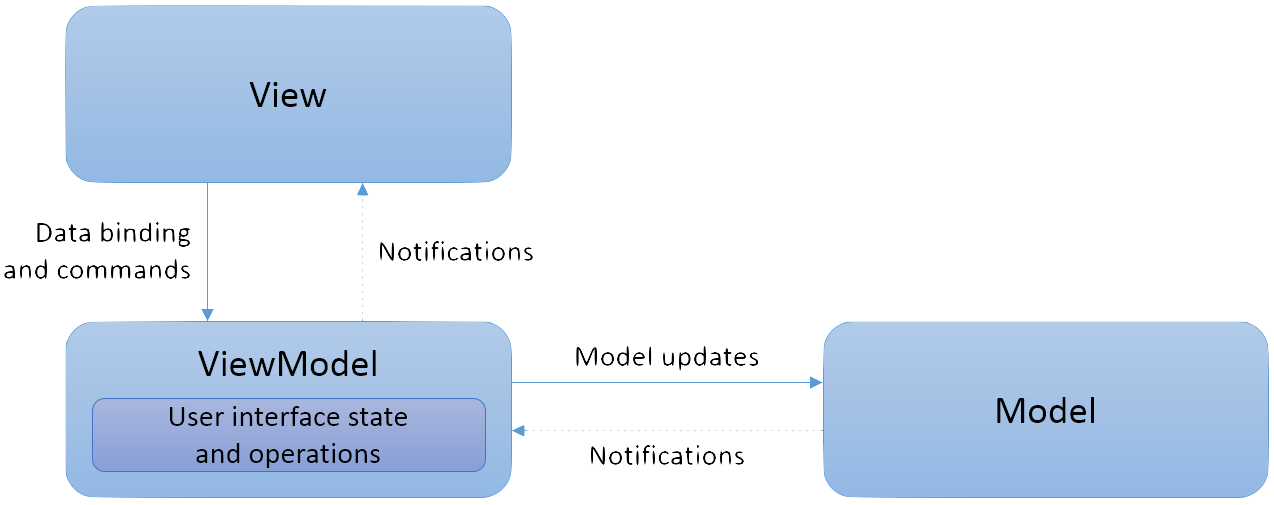
\includegraphics[scale=0.4]{img/mvvm.png}
		\caption{MVVM}
		
	\end{figure}
\end{frame}


\section{Front-End}

\newpage
\subsection{Back-end}

Il lato back-end risulta così strutturato:

\begin{figure}[H]
	\centering
	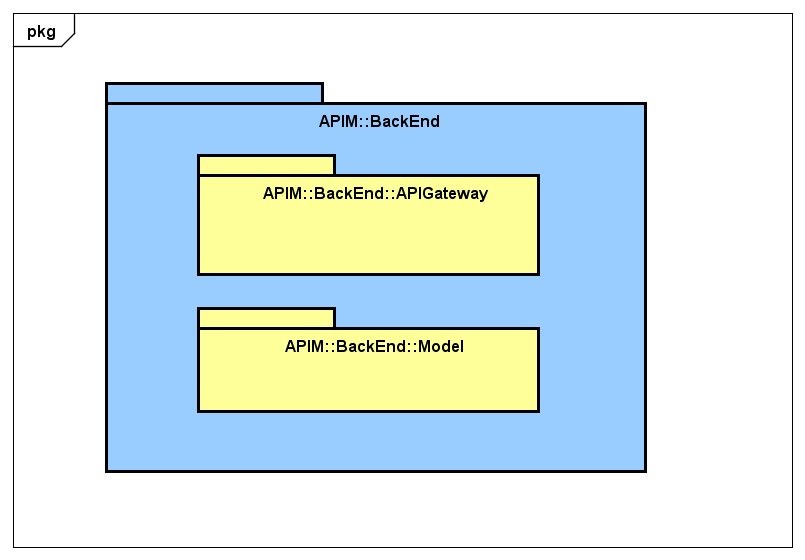
\includegraphics
	[width=0.7\linewidth]
	{UML/DiagrammiPackage/BackEnd.png}
	\caption{Package APIM::BackEnd}
\end{figure}

Nella parte back-end sono dunque presenti i package APIGateway e Model strutturati secondo un'architettura a microservizi.


\begin{figure}[H]
	\centering
	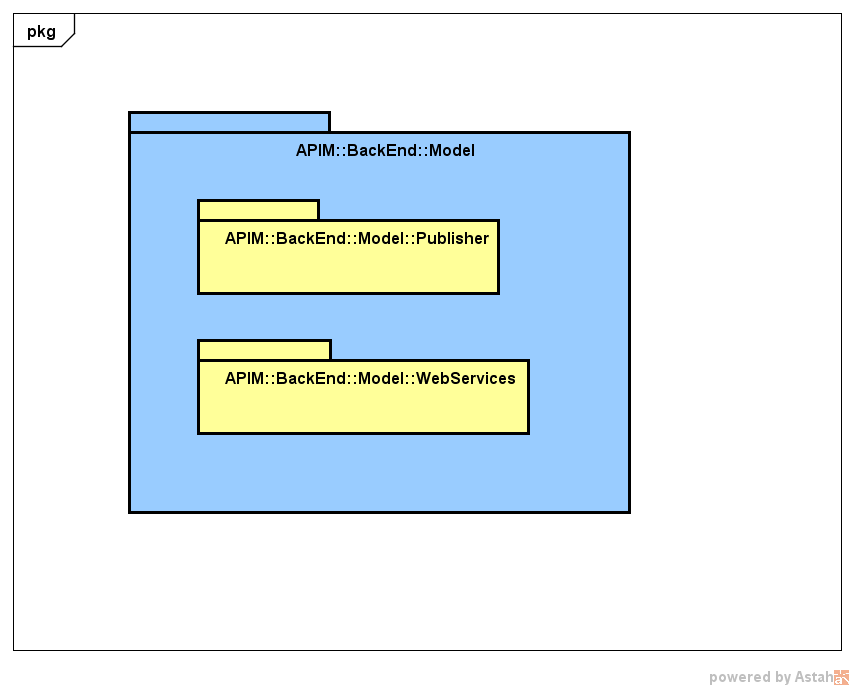
\includegraphics
	[width=0.7\linewidth]
	{UML/DiagrammiPackage/Model.png}
	\caption{Package APIM::BackEnd::Model}
\end{figure}

Il package \textit{Model} contiene i packages utilizzati per rappresentare i dati e l'implementazione della logica di business e di validazione.
\begin{itemize}
	\item \textbf{Publisher}: contiene le classi per la pubblicazione dei dati;
	\item \textbf{WebServices}: contiene le classi per la comunicazione col database.
\end{itemize}


\subsubsection{Publisher}
\begin{figure}[H]
	\centering
	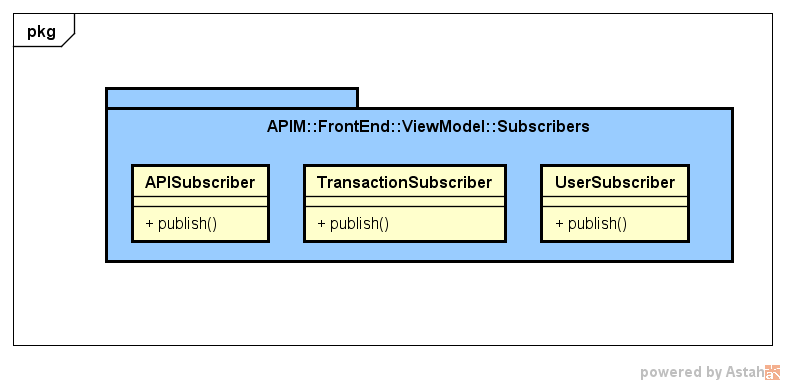
\includegraphics
	[width=0.7\linewidth]
	{UML/DiagrammiPackage/Publisher.png}
	\caption{Package APIM::BackEnd::Model::Publisher}
\end{figure}

Il package \textit{Publisher} contiene le classi necessarie ad esporre il modello dati al front-end.

\paragraph{APIPublisher}
\begin{itemize}
	\item \textbf{Funzione del componente}: esegue la pubblicazione delle API;
	\item \textbf{Attività svolte e dati trattati}: permette l'accesso alla collezione di API.
\end{itemize}

\paragraph{TransactionPublisher}
\begin{itemize}
	\item \textbf{Funzione del componente}: esegue la pubblicazione delle transazioni;
	\item \textbf{Attività svolte e dati trattati}: permette l'accesso alla collezione di transazioni.
\end{itemize}

\paragraph{UserPublisher}
\begin{itemize}
	\item \textbf{Funzione del componente}: esegue la pubblicazione degli utenti;
	\item \textbf{Attività svolte e dati trattati}: permette l'accesso alla collezione di utenti.
\end{itemize}


\subsubsection{WebServices}

\begin{figure}[H]
	\centering
	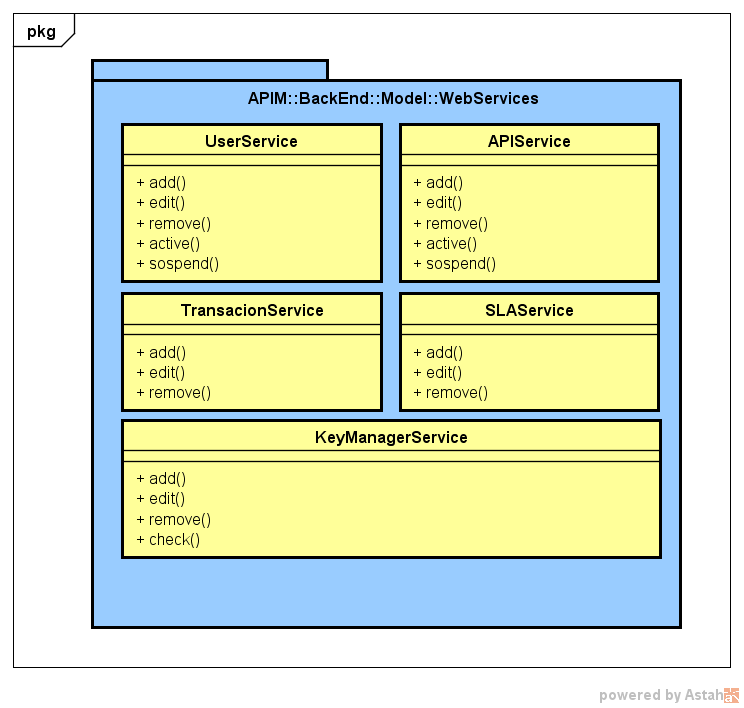
\includegraphics
	[width=0.7\linewidth]
	{UML/DiagrammiPackage/WebServices.png}
	\caption{Package APIM::BackEnd::Model::WebServices}
\end{figure}

Il package \textit{WebServices} contiene i microservizi utilizzati per mettere in comunicazione il database con il \textit{Model}.

\paragraph{UserService}
\begin{itemize}
	\item \textbf{Funzione del componente}: esegue le funzioni di inserimento, modifica e rimozione di utenti;
	\item \textbf{Relazioni d'uso di altri componenti}: si interfaccia con il \textit{ViewModel} e il database per fornire le funzioni di inserimento, modifica e rimozione di utenti.
\end{itemize}

\paragraph{APIService}
\begin{itemize}
	\item \textbf{Funzione del componente}: esegue le funzioni di inserimento, modifica e rimozione di API;
	\item \textbf{Relazioni d'uso di altri componenti}: si interfaccia con il \textit{ViewModel} e il database per fornire le funzioni di inserimento, modifica e rimozione di API.
\end{itemize}

\paragraph{TransactionService}
\begin{itemize}
	\item \textbf{Funzione del componente}: esegue le funzioni di inserimento, modifica e rimozione di transazioni;
	\item \textbf{Relazioni d'uso di altri componenti}: si interfaccia con il \textit{ViewModel} e il database per fornire le funzioni di inserimento, modifica e rimozione di transazioni.
\end{itemize}


\paragraph{SLAService}
\begin{itemize}
	\item \textbf{Funzione del componente}: esegue le funzioni di inserimento, modifica e rimozione di log di SLA;
	\item \textbf{Relazioni d'uso di altri componenti}: si interfaccia con il \textit{ViewModel} e il database per fornire le funzioni di inserimento, modifica e rimozione di log di SLA.
\end{itemize}

\paragraph{KeyManagerService}
\begin{itemize}
	\item \textbf{Funzione del componente}: esegue le funzioni di inserimento, modifica e rimozione di API key;
	\item \textbf{Relazioni d'uso di altri componenti}: si interfaccia con il \textit{ViewModel} e il database per fornire le funzioni di inserimento, modifica e rimozione di API key.
\end{itemize}


\newpage
\section{API Gateway}





\section{Piano di Qualifica}

\section{Piano di Progetto}









\end{document}